\documentclass{minimal}
\usepackage{tikz}
%% \usepackage{pgfmath}

\begin{document}

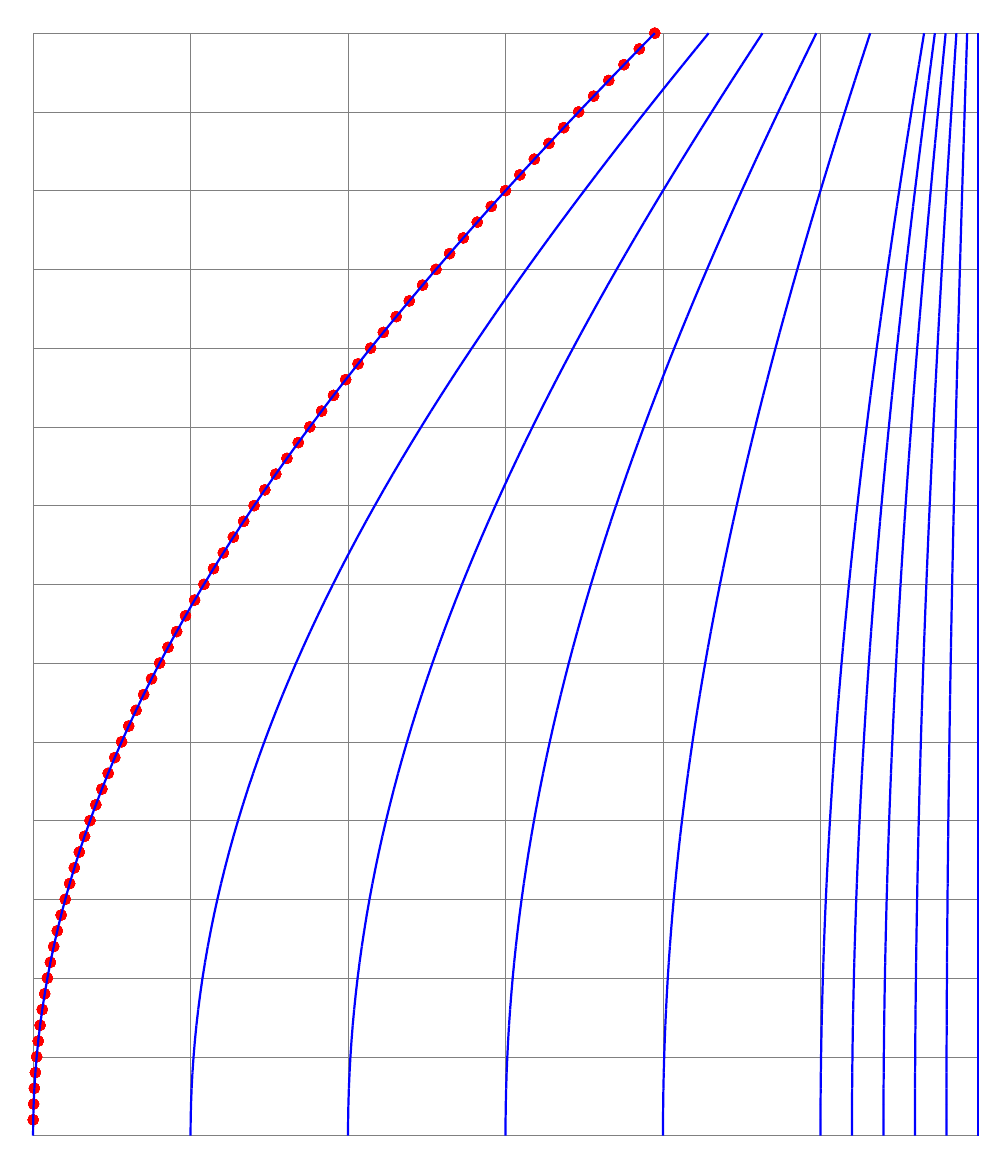
\begin{tikzpicture}[domain=0:60, scale=0.2]
  \draw[very thin,color=gray,xstep=10,ystep=5] (60,0) grid (0,70);
  \foreach \y in {1,...,70} {
    \foreach \step in {0,2,...,10,20,30,40,50,60} {
      
      \fill[red] ({sin(90-\y)*-60+60},\y) circle [radius=10pt];
      \draw[blue, thick] ({sin(90-\y)*-\step+60},\y) -- ({sin(90-\y+1)*-\step+60},\y-1);
    }
  }
\end{tikzpicture}

\end{document}
